\documentclass{article}
\usepackage[utf8]{inputenc}
\usepackage{graphicx}
\usepackage[american]{circuitikz}
\usepackage{karnaugh-map}
\usepackage{float}
\usepackage{xcolor}
\usepackage{listings}
\usepackage{enumitem}

\definecolor{mGreen}{rgb}{0,0.8,0}
\definecolor{mGray}{rgb}{0.5,0.2,0.5}
\definecolor{mPurple}{rgb}{0.5,0,0.82}
\definecolor{backgroundColour}{rgb}{0.9,0.95,0.92}

\lstdefinestyle{CStyle}{
    backgroundcolor=\color{backgroundColour},   
    commentstyle=\color{mGreen},
    keywordstyle=\color{magenta},
    numberstyle=\tiny\color{mGray},
    stringstyle=\color{mPurple},
    basicstyle=\footnotesize,
    breakatwhitespace=false,         
    breaklines=true,                 
    captionpos=b,                    
    keepspaces=true,                 
    numbers=left,                    
    numbersep=5pt,                  
    showspaces=false,                
    showstringspaces=false,
    showtabs=false,                  
    tabsize=2,
    language=C
}

\title{Digital Logic Design Assignment 9 - EC2018-31}
\author{Priyansh Agrahari}

\begin{document}

\maketitle

\section{Question:}
\textbf{A four-variable Boolean function is realized using 4x1 multiplexers as shown in the figure:}
\vspace{1cm}
\begin{center}
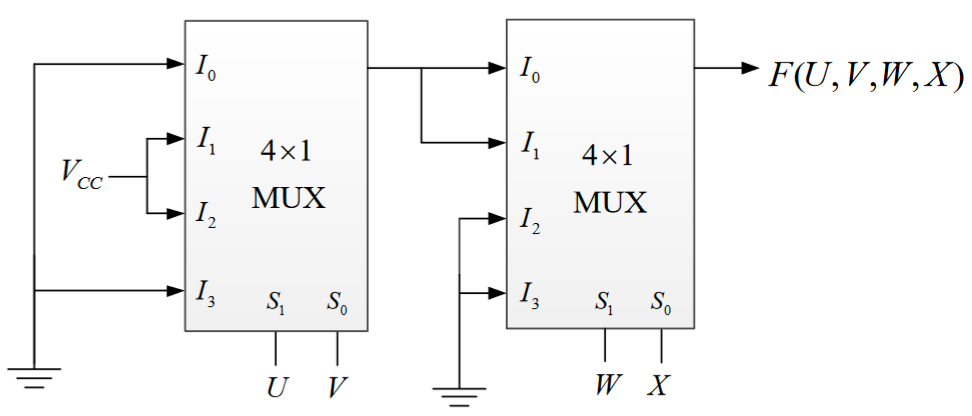
\includegraphics[scale=0.3]{images/MUX_fig.png}
\end{center}
\vspace{1cm}
\textbf{The minimized expression for F(U,V,W,X) is}
\begin{enumerate}[label=(\Alph*)]
\item $(U$ $V$ + $\overline{U}$  $\overline{V}$) $\overline{W}$
\item ($U$ $V$ + $\overline{U}$ $\overline{V}$) ($\overline{W}$  $\overline{X}$ + $\overline{W}$ $\overline{X}$)
\item ($U$ $\overline{V}$ + $\overline{U}$ $V$) $\overline{W}$
\item ($U$ $\overline{V}$ + $\overline{U}$ $V$) ($\overline{W}$ $\overline{X}$ + $\overline{W}$ $X$)
\end{enumerate}

\pagebreak{}

\section{Solution:}
\begin{figure}[!h]\centering
%\hspace{5cm}
\begin{circuitikz}
    \ctikzset{tripoles/american nand port/height=1.5};
    \draw
    (0,0)node[nand port,number inputs=3](i3){}
    (0,2.5)node[nand port,number inputs=3](i2){}
    (0,5)node[nand port,number inputs=3](i1){}
    (0,7.5)node[nand port,number inputs=3](i0){}
    ;
    \ctikzset{tripoles/american nand port/height=2};
    \draw(3,3.8)node[nand port,number inputs=4](out){};
    \draw
    (i0.in 1)node[anchor=east]{$I_0$}
    (i0.in 2)node[anchor=east]{$U$}
    (i0.in 3)node[anchor=east]{$V$}
    (i1.in 1)node[anchor=east]{$I_1$}
    (i1.in 2)node[anchor=east]{$U$}
    (i1.in 3)node[anchor=east]{$V$}
    (i2.in 1)node[anchor=east]{$I_2$}
    (i2.in 2)node[anchor=east]{$U$}
    (i2.in 3)node[anchor=east]{$V$}
    (i3.in 1)node[anchor=east]{$I_3$}
    (i3.in 2)node[anchor=east]{$U$}
    (i3.in 3)node[anchor=east]{$V$}
    (out.out)node[anchor=west]{$Output$}
    
    (i0.out)--(out.in 1)
    (i1.out)--(out.in 2)
    (i2.out)--(out.in 3)
    (i3.out)--(out.in 4)
    ;
    \node at (i0.bin 2)[ocirc,left]{};
    \node at (i0.bin 3)[ocirc,left]{};
    \node at (i1.bin 2)[ocirc,left]{};
    \node at (i2.bin 3)[ocirc,left]{};
\end{circuitikz}
\caption{$Logic$ $circuit$ $equivalent$ $of$ 4x1 $MUX$ $used$ $to$ $solve$ $this$ $problem$}
\end{figure}
Since we have $I_0$ and $I_3$ grounded, we can take their boolean equivalents to be 0. Then, we get the following equation:
\begin{equation}
    Output = \overline{ (U + \overline{V}) (\overline{U} + V) }
\end{equation}
which can be further simplified (using de Morgan's law) to obtain:
\begin{equation}
    Output = U \overline{V} + \overline{U} V
\end{equation}
\hspace{0.5cm}
Moving further, the same logic can be used to obtain the result of the second MUX. Since in this case, $I_2$ and $I_3$ are grounded; hence by taking their boolean equivalents to be 0, we get the following equation from the second MUX:
\begin{equation}
    F = \overline{ \overline{(Output. \overline{W}. \overline{X})}. \overline{(Output. \overline{W}. X )}}
\end{equation}
simplifying, we get:
\begin{equation}
    F = Output.\overline{W}.\overline{X} + Output.\overline{W}.X
\end{equation}
after placing the value of $Output$ from eq.(2), and performing a few more manipulations, we get:
\begin{equation}
    F = (U\overline{V}+\overline{U}V)\overline{W}(X+\overline{X})
\end{equation}
\hspace{0.5cm}
Since $X$+$\overline{X}$=1, we finally get the desired equation:
\begin{equation}
    F = (U\overline{V}+\overline{U}V)\overline{W}
\end{equation}
Hence, the answer the given question is (C).

\vspace{5cm}

\section{Truth Table}
\begin{table}[H]
\centering
\begin{tabular}{|c|c|c|c|c|c|}
\hline
\textit{\textbf{U}} & \textit{\textbf{V}} & \textit{\textbf{W}} & \textit{\textbf{X}} & \textit{\textbf{F}} & \textbf{Term}    \\ \hline
0                   & 0                   & 0                   & 0                   & 0                   & -                \\
0                   & 0                   & 0                   & 1                   & 0                   & -                \\
0                   & 0                   & 1                   & 0                   & 0                   & -                \\
0                   & 0                   & 1                   & 1                   & 0                   & -                \\
0                   & 1                   & 0                   & 0                   & 1                   & \textit{$\overline{U}$ V $\overline{W}$  $\overline{X}$} \\
0                   & 1                   & 0                   & 1                   & 1                   & \textit{$\overline{U}$ V $\overline{W}$ X}  \\
0                   & 1                   & 1                   & 0                   & 0                   & -                \\
0                   & 1                   & 1                   & 1                   & 0                   & -                \\
1                   & 0                   & 0                   & 0                   & 1                   & \textit{U $\overline{V}$ $\overline{W}$ $\overline{X}$} \\
1                   & 0                   & 0                   & 1                   & 1                   & \textit{U $\overline{V}$ $\overline{W}$ X}  \\
1                   & 0                   & 1                   & 0                   & 0                   & -                \\
1                   & 0                   & 1                   & 1                   & 0                   & -                \\
1                   & 1                   & 0                   & 0                   & 0                   & -                \\
1                   & 1                   & 0                   & 1                   & 0                   & -                \\
1                   & 1                   & 1                   & 0                   & 0                   & -                \\
1                   & 1                   & 1                   & 1                   & 0                   & -                \\ \hline
\end{tabular}
\caption{Truth Table for eq.(6)}
\label{tab:my-table}
\end{table}

\section{K-map for the function F(U,V,W,X)}
\hspace{2cm}
\begin{center}
\begin{karnaugh-map}[4][4][1][][]
    \maxterms{0,3,4,7,8,9,10,11,12,13,14,15}
    \minterms{1,5,2,6}
    
    \implicant{1}{5}
    \implicant{2}{6}

    \draw[color=black, ultra thin] (0, 4) --
    node [pos=0.7, above right, anchor=south west] {$UV$}
    node [pos=0.7, below left, anchor=north east] {$WX$}
    ++(135:1);
\end{karnaugh-map}
\end{center}
The expression obtained using the K-map is the same as the one obtained earlier in eq.(6). Alternatively, we can also make a K-map for obtaining the POS expression:
\hspace{2cm}
\begin{center}
\begin{karnaugh-map}[4][4][1][][]
    \maxterms{0,3,4,7,8,9,10,11,12,13,14,15}
    \minterms{1,5,2,6}
    
    \implicant{0}{8}
    \implicant{3}{11}
    \implicant{12}{10}

    \draw[color=black, ultra thin] (0, 4) --
    node [pos=0.7, above right, anchor=south west] {$UV$}
    node [pos=0.7, below left, anchor=north east] {$WX$}
    ++(135:1);
\end{karnaugh-map}
\end{center}
The POS expression hence obtained is:
\begin{equation}
    F = (U+V)(\overline{U}+\overline{V})\overline{W}
\end{equation}

\pagebreak{}

\section{C implementation to verify Table 1}
\subsection{C code:}
\begin{lstlisting}[style=CStyle]
#include <stdio.h>
int main(void)
{
   unsigned char U = 0x00, V = 0x01, W = 0x00, X = 0x00;
   unsigned char F, one = 0x01;
   
   F = (~W) & ( (U & (~V)) | ((~U) & V) );
   printf("Using SOP form: F = %x\n", (F & one));
   
   F = (U | V) & ((~U) | (~V)) & (~W);
   printf("Using POS form: F = %x\n", (F & one));
}
\end{lstlisting}
\subsection{Output:}
\begin{lstlisting}[style=CStyle]
Using SOP form: F = 1
Using POS form: F = 1
\end{lstlisting}

\hline

\end{document}
